\section{Unfolding methods}
\label{sec:UnfoldingMethods}

As introduced in Section~\ref{sec:Introduction}, after the discovery of the Higgs boson at CERN, it becomes even more important to test the validity of the SM via precision measurements on SM particles. Properties of such particles are measured in the ATLAS detector. The measured quantities are close, but not identical to the true value of the quantities these particles had in reality in nature, due to detector smearing effects. Every measurement has a total uncertainty, formed from statistical and systematic uncertainties. It is therefore important to have a mechanism to reverse the detector smearing by inferring the true value of a quantitity given the measured value of the quantity. Such mechanism is called \emph{unfolding} and is the topic of this project. The estimated true quantity from unfolding the reconstructed quantity is then compared with the theoretical prediction. If a difference is observed even after taking into account the experimental and theoretical uncertainties, a deviation from the SM would be observed. If confirmed at five standard deviations ($\sigma$), it would represent a revolution in particle physics. Therefore, unfolding methods are key to testing the SM and searching for new physics beyond the Standard Model (BSM). An introduction to unfolding methods for particle physics can be studied in~\cite{UnfoldingStatSchool}.

\ \\There are two types of unfolding methods: a traditional method using a binned 2D hisogram representing a migration matrix for one variable, and machine learning predicting a continuous function for several variables, as illustrated in Figure~\ref{fig:TwoUnfoldingTechniques}. 

\begin{figure}[t]
  \centering
  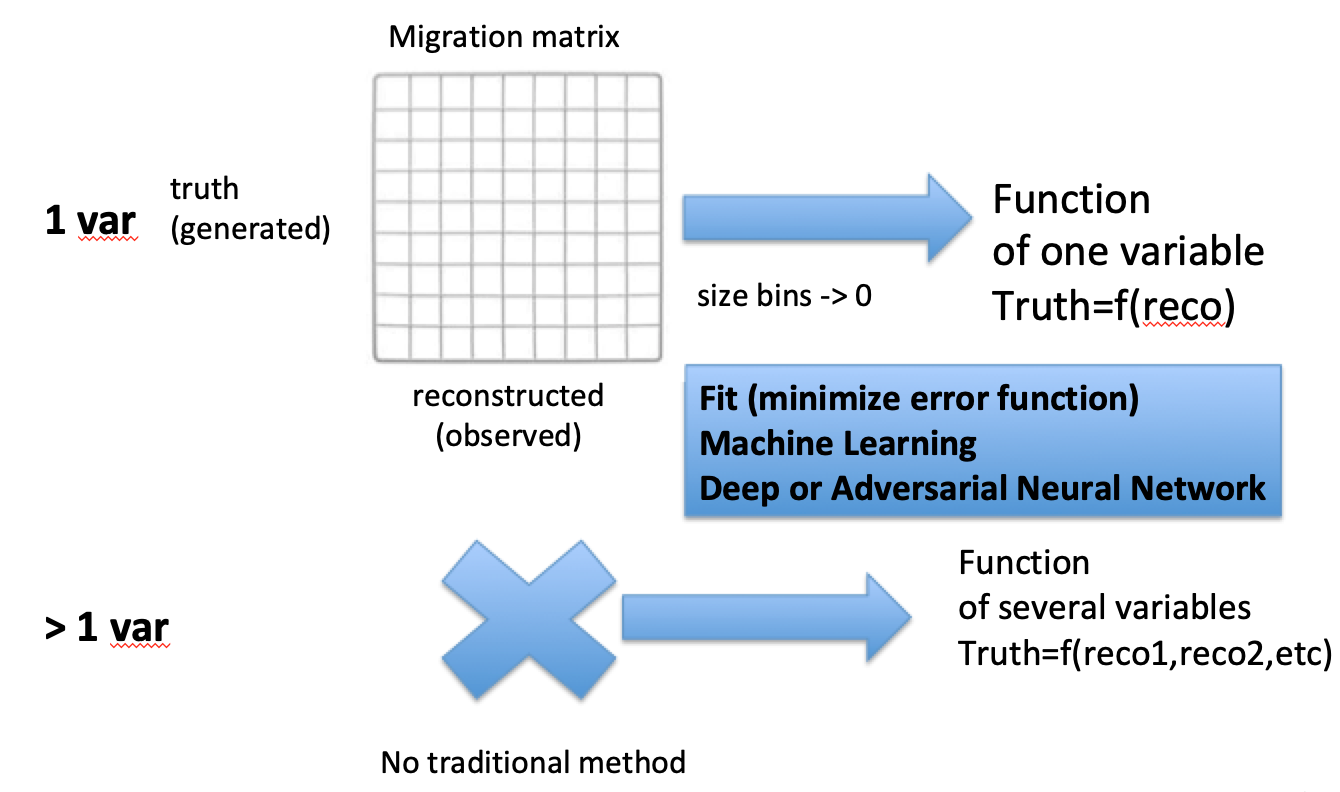
\includegraphics[width=0.98\textwidth]{../presentation/plots/Unfolding_Traditional_ML.png}
  \caption{Comparison of the two unfolding method: traditional (migration matrix, one variable) and machine learning (continuous function, several variables).}
  \label{fig:TwoUnfoldingTechniques}
\end{figure}

\subsection{The traditional method: the migration matrix}
\label{sec:UnfoldingMigrationMatrix}

In the traditional method, only one quantity is used at a time. In simulated data, there are two versions for each quantity of the same event: a reconstructed quantity (or reco, which for measured data would be the observed quantity) and the generated quantity (that would be the truth, or the true value in nature). An interval and binning is chosen for this variable. A 2D histogram is filled, as a given event is in a particular bin in the reco on the horizontal and in a particular bin in the truth on the vertical. The histogram is called a migration matrix, as it describes how a quantity migrates from a particular bin in the reconstructed to another bin (usually nearby) for the truth. Ideally, this matrix is diagonal. In practice, there are non diagonal values that are non zero. Such a matrix is used in the traditional unfolding. 

\ \\For the simulated dataset studied in this report, the migration matrix of the leading jet \pt~bin value is presented in Figure~\ref{fig:MigrationMatrix}, taken from~\cite{ReportYichenLi}. There are 25 bins possible for the leading jet \pt~values between 0 and 500 \GeV, with 20 \GeV~bins. The number in a cell represents the probability (as a percent) of an event in the truth bin \emph{i} to be reconstructed in a reco bin \emph{j}. The numbers are normalised so that the sum of values on a horizonthal row is 100 (percent). The more diagonalizable matrix, the easier unfolding will be. Events are migrating from one truth bin to other bins for reco, and vice-versa.

\begin{figure}[h]
  \centering
  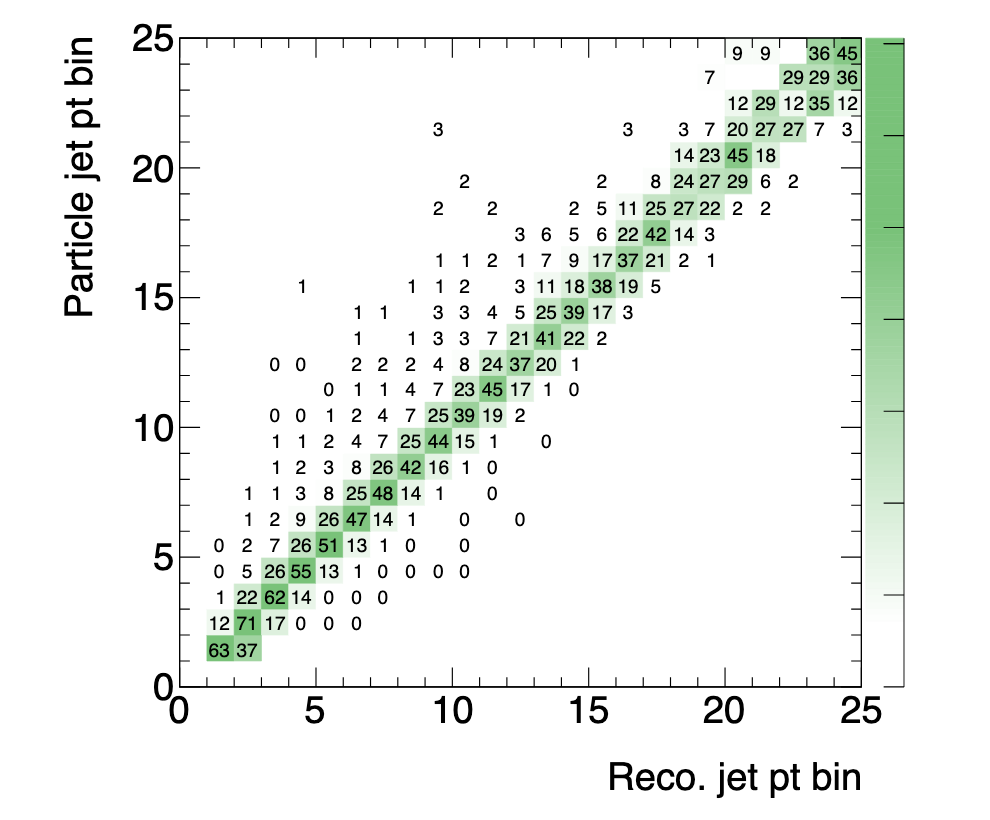
\includegraphics[width=0.8\textwidth]{../presentation/plots/jetPt_migration_matrix.png}
  \caption{The leading particle jet \pt~bin versus the leading reco jet \pt~bin, for the same events of this study~\cite{ReportYichenLi}.}
  \label{fig:MigrationMatrix}
\end{figure}

\ \\Traditional unfolding is an iterative Bayesian process. After four iterations, the unfolded results are presented in Figure~\ref{fig:2DMigrationMatrix}, taken from~\cite{ReportYichenLi}. The left hand-side presents the jet distribution for truth and for the truth unfolded from the reco, while the right-hand side presents the coefficients matrix in a 2D histogram format.

\begin{figure}[h]
  \centering
  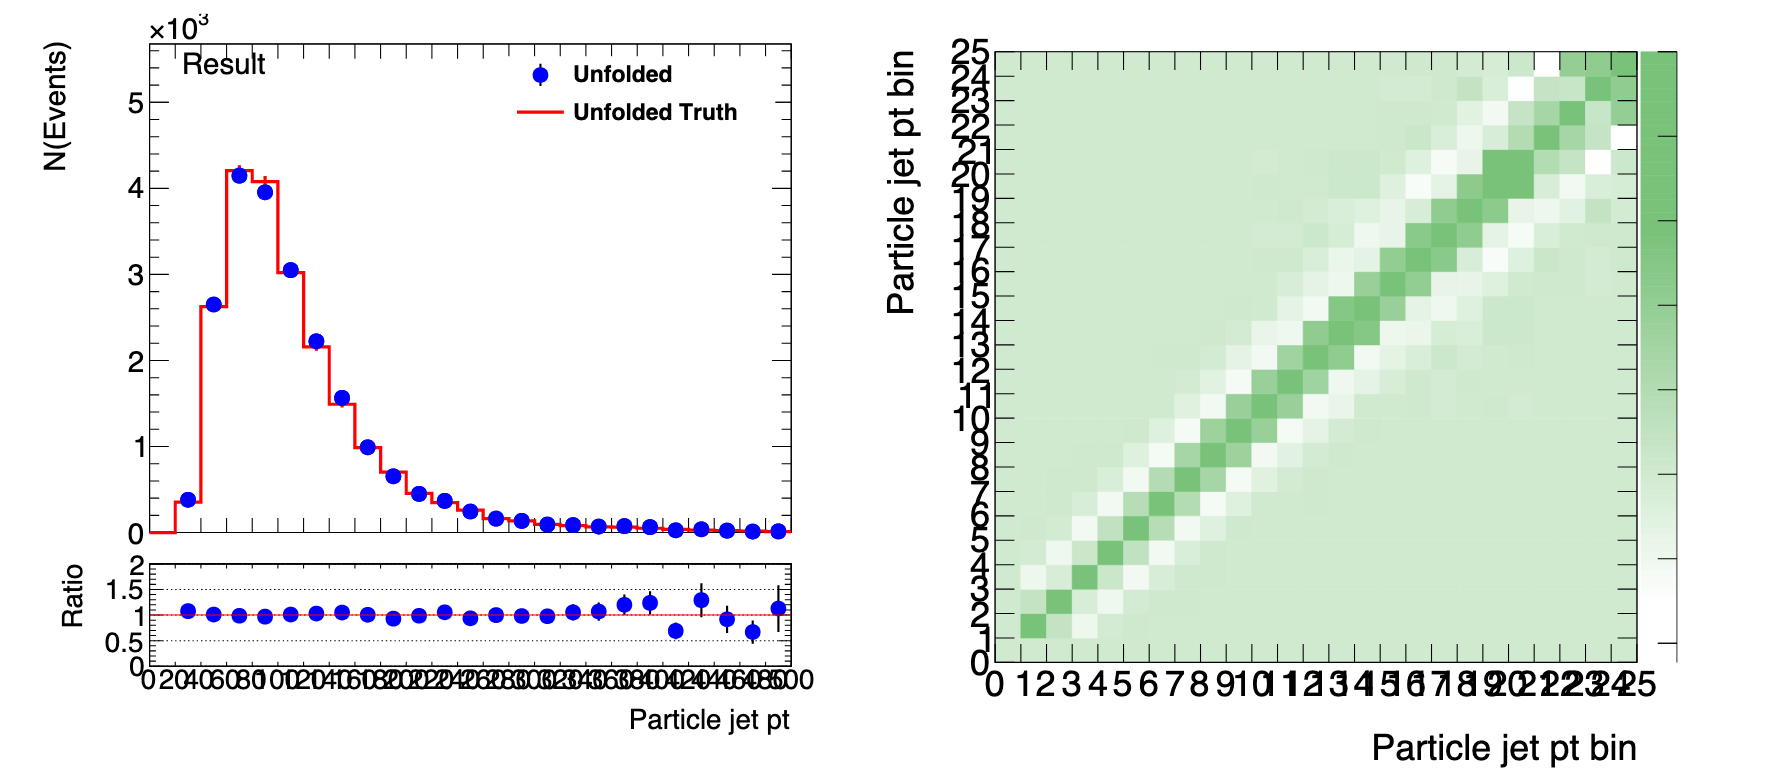
\includegraphics[width=0.98\textwidth]{./plots/TraditionalUnfoldingResults.png}
  \caption{Traditional unfolding results for the leading jet \pt~in a 1D and 2D histogram.}
  \label{fig:2DMigrationMatrix}
\end{figure}

\subsection{The new method: machine learning}
\label{sec:UnfoldingMachine Learning}

As the bin width is decreased continuously closed to infinitesimal values, the migration matrix becomes a function of one variable that maps each reco quantity to its truth quantity. This is equivalent to a function \texttt{truth=f(reco)}. But it still can have only one variable. Finding such a function is in general found via minimizing an error function over some parameter space, a process which is also called a \emph{fit}. A fit with even several variables can be done successfully via machine learning, where a functions is learned of the form \texttt{truth=f(reco1, reco2, etc.)}. 

\ \\A new approach of unfolding via machine learning has been proposed by A. Glazov at DESY Hamburg~\cite{AGlazov}, together with a code example~\cite{AGlazovCode} of training a (deep) neural network on toy simulated data using TensorFlow~\cite{TensorFlow} via ~\cite{Keras} in \texttt{Python}, using numpy~\cite{numpy}, as illustrated in Figure~\ref{fig:CodeSoftware}. 

\begin{figure}[h]
  \centering
  
\includegraphics[width=0.30\textwidth]{../presentation/plots/TensorFlow_Keras.png}
  
\includegraphics[width=0.30\textwidth]{../presentation/plots/Python.png}
  \caption{A modern (deep) neural network is typically trained in Keras with a TensorFlow backend, run in Python, using numpy.}
  \label{fig:CodeSoftware}
\end{figure}

\ \\The goal of the study is to adapt this example to use real data coming from the jet \pt~distribution from the \ttbaremu~analysis. We use this \texttt{.root} flat tree~\cite{RootFile}. This file contains both the reconstructed and truth jets, already matched. Meaning the i$^{\rm th}$ event from reco, corresponds to the i$^{\rm th}$ event from truth. Each jet collection contains jets already the jets ranked by \pt. We take index 0 to consider the leading reco jet and the leading truth jet.

\ \\Using this approach, the leading jet \pt~unfolding is formulated in the example illustrated in Figure~\ref{fig:PhysicsProblem}. For both reco and truth, \pt~larger than 500 \GeV~are changed to 499.999 \GeV, and thus moved to the last bin. This is equivalent to moving the overflow bin of a histogram to the last bin of a histogram. The truth and reco are thus ensured to have the same number of potential bins (25), given the 0-500 \GeV~range and the bin width of 20 \GeV. The simplest case of only one variable is considered: the jet \pt, or more exactly, the jet \pt~bin. Let's consider an example for the reconstructed jet (the input of unfolding) and the truth jet (the output of unfolding).

\begin{figure}[h]
  \centering
  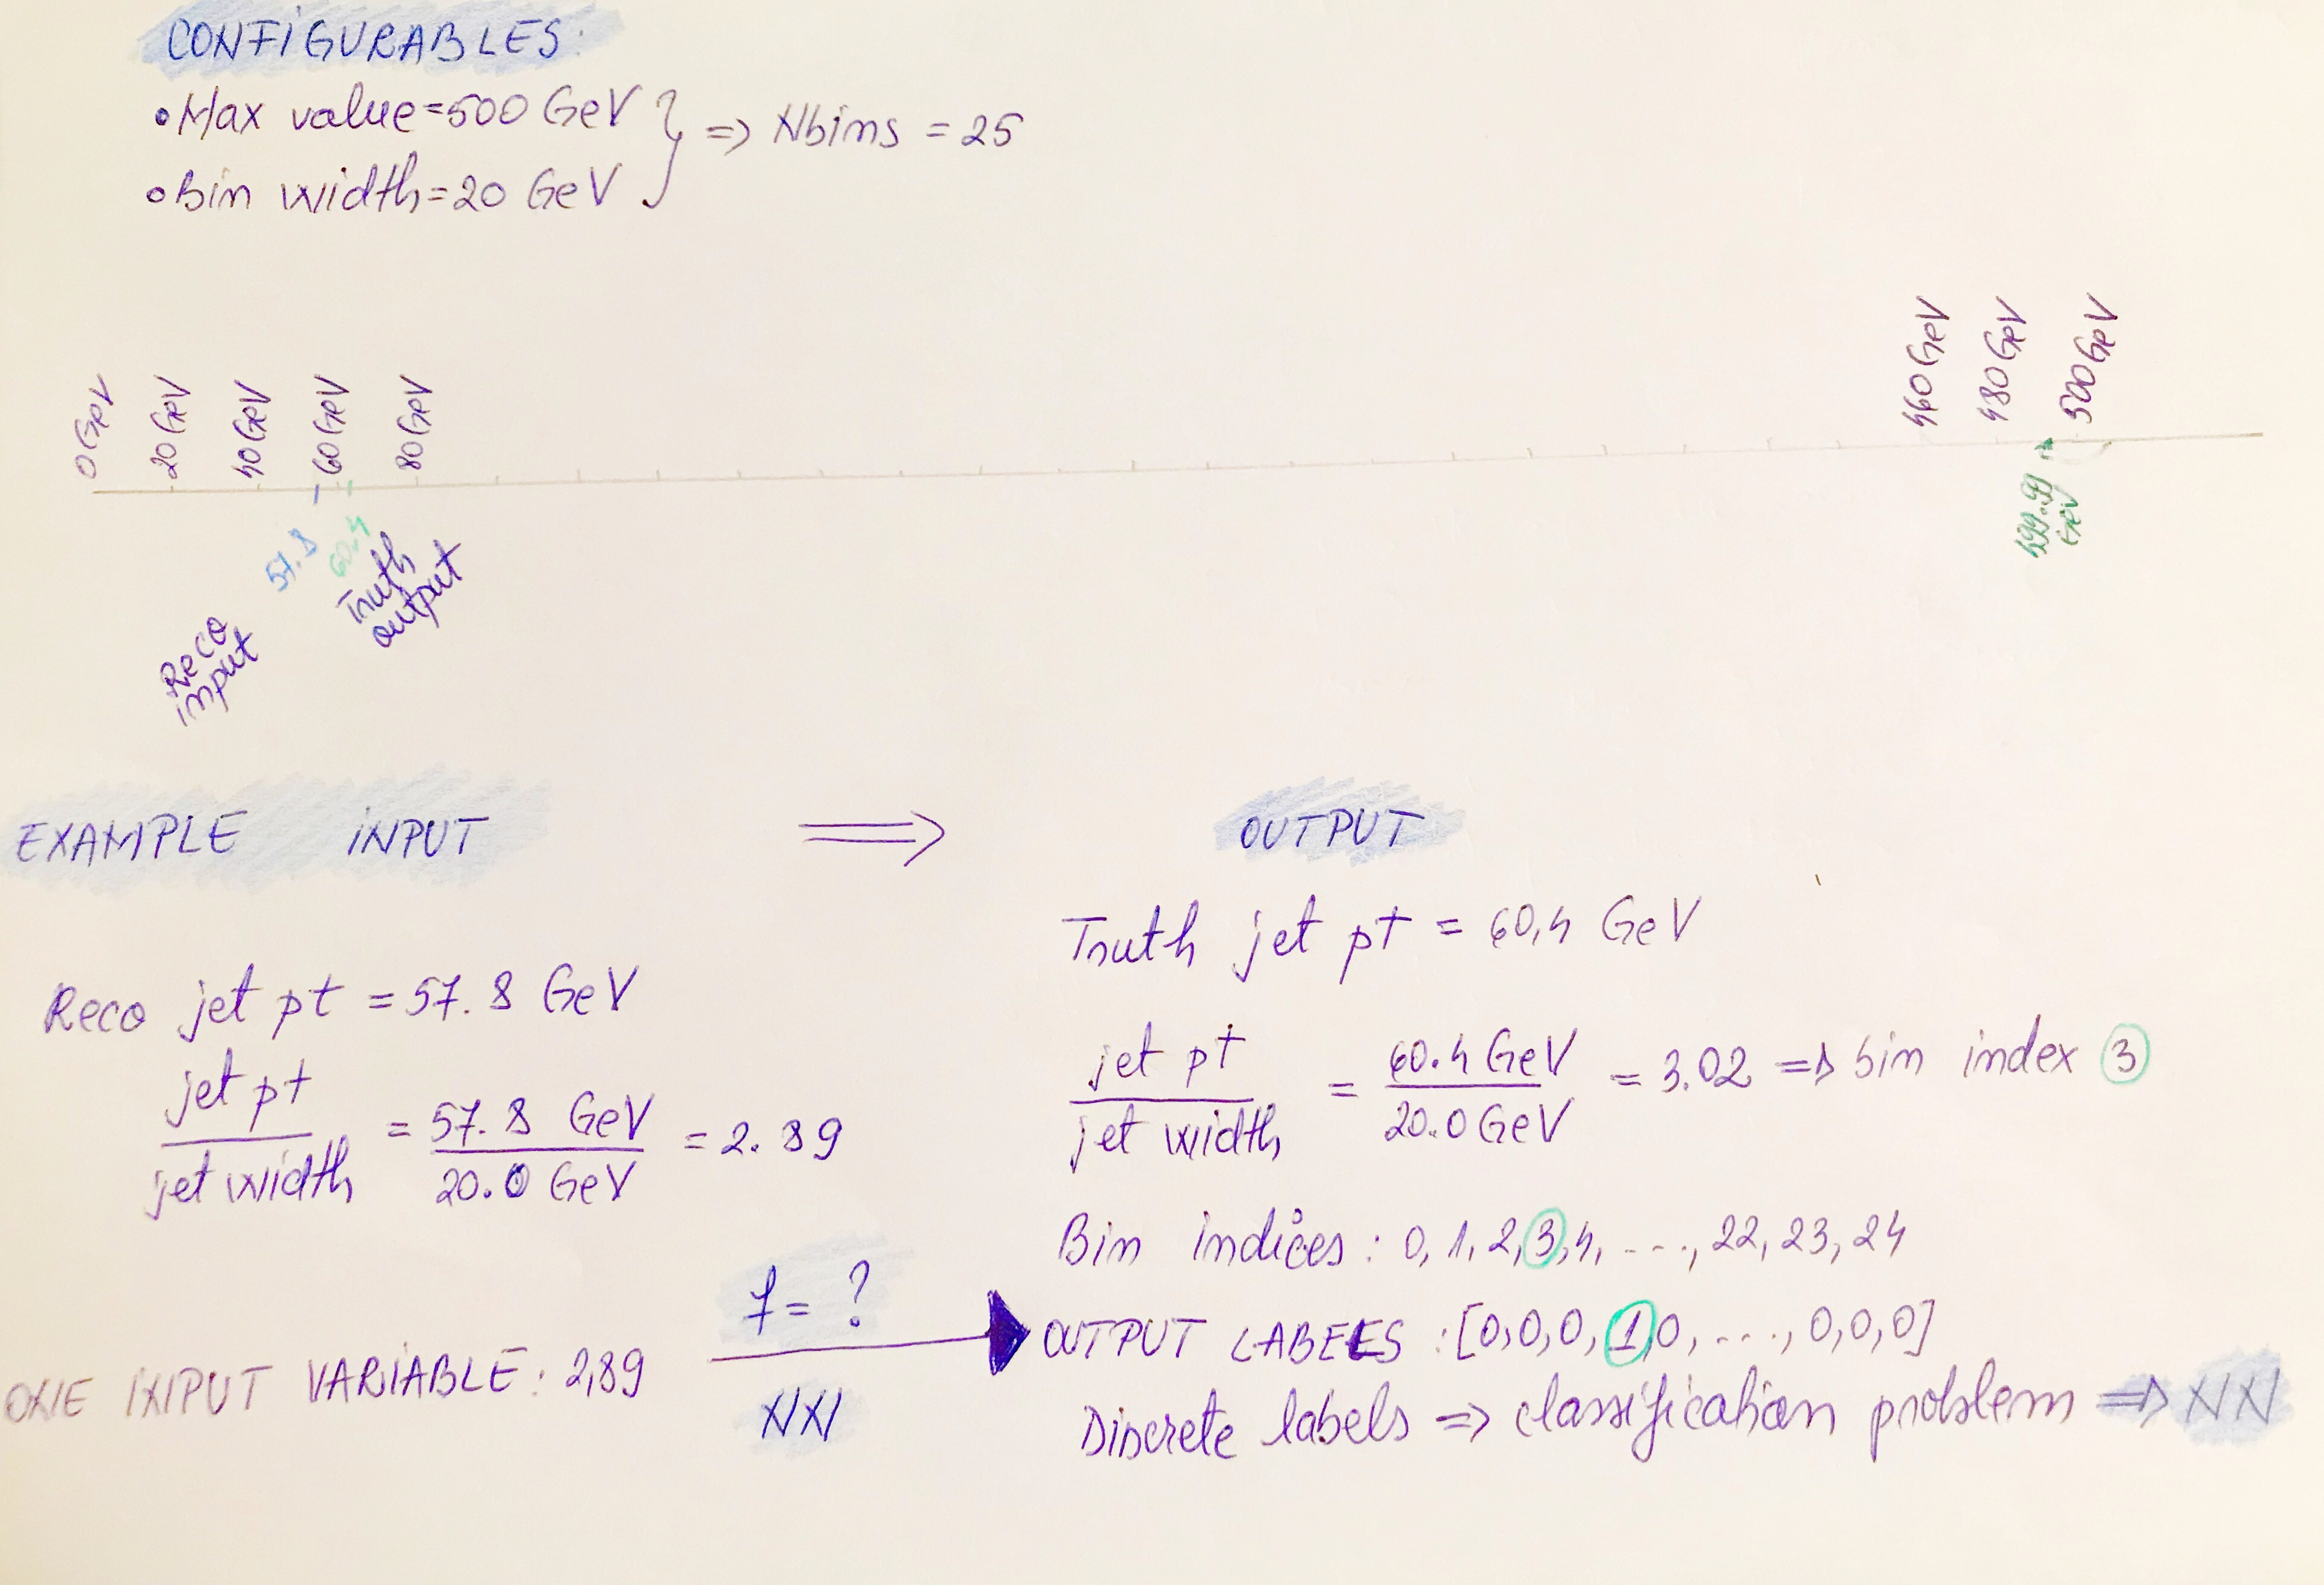
\includegraphics[width=0.98\textwidth]{../presentation/plots/PhysicsProblem.jpg}
  \caption{Exemple of problem posing for the leading jet \pt~unfolding with the machine learning approach of~\cite{AGlazov}~\cite{AGlazovCode}.}
  \label{fig:PhysicsProblem}
\end{figure}

\ \\For a reconstructed jet, the ratio between the \pt and the bin width represents the input to the machine learning. For example, for a 57.8 \GeV~jet, the value is 2.89. The jet would fit in the third bin, or the bin of index 2 (index values start at 0).

\ \\For a truth jet, things are similar, but a bit more complex. Imagine the same jet has a different value for the truth, equal with 60.4 \GeV. Dividing by the bin width, 3.02 is obtained. The truth jet falls in the fourth bin, or the bin of index 3. The goal of the unfolding via machine learning is to learn and then predict, or infer, this number 3. 3 is only one possible answer out of finate number of posibilities corresponding to the 25 bins. Each bin can be considered one category of potential output. Each jet belongs to only one category. This problem is called classification and can indeed be solved via machine learning. To note that in this method is not attempted to predict exactly the \pt~of the truth jet. There would be a continous interval of possible values. Such a problem is called regression. It is also possible to be solved via machine learning, but it is more complex. 

\ \\In this project we choose to predict only the bin where the jet \pt~falls into, or a multi-label classification or categorization problem. The categorisation is a common problem solved via modern Machine Learning methods. Possible methods could be Boosted Decision Trees (BDT)~\cite{JoshuaBendavid}~\cite{AndrewNg} and Artificial Neural Networks (ANN or NN)~\cite{AndrewNg}. 

\ \\Classification is usually binary, distinguishing between two possibilties: signal or background, good or bad, 1 or 0. It is therefore technically easier to formulate that for the input of 2.89, the output not as the bin index 3, but as a range of 25 values, each being 0 or 1, all of them being zero, except for the index 3, where the value is 1, as illustrated in Table~\ref{tab:InputOutput}. Finding such a function connecting this type of input to this type of output for all the jets in the event is done via a deep neural network (NN) training in this project. The NN will try to learn and predict for each of the 25 positions the values of 0 or 1. But in practice it will output for each position a real number with a value between 0.0 and 1.0. The NN will return the probability that for a given jet its \pt~falls in any of these bins. The total probability for all bins must be 1.

\begin{table}[h!]
  \centering
    \begin{tabular}{|l|l|l|}
      \hline
      \textbf{Jet} & \textbf{Input} & \textbf{Output}\\
      \hline
      Physics & 2.89 & 3.02 \\
      Classification & 2.89 & 3 \\
      Neural Network & 2.89 & [0,0,0,1,0,0,...,0,0,0] \\
      \hline
    \end{tabular}
 \caption {Example of jet reco (input) and truth (output) from physics to the NN.}
\label{tab:InputOutput}
\end{table}

\ \\The input and output layers of the NN are fixed by the problem formulation. The architecture of the middle layers can be optimised for the specific problem. The NN architecture suggested in the code example~\cite{AGlazovCode} is denoted in this report the old NN. Several architectures and NN hyper-parameters have been optimised in this study by changing one parameter while keeping all the rest constant. The best of the many NNs tried is denoted in this report the new NN. 

\ \\The following section~\ref{sec:NeuralNetworks} will describe the optimisation process and compare the two NNs in terms of the NN-specific figures of merits of accuracy and loss. After that, the section~\ref{sec:Results} will compare the two NNs in terms of the unfolding of the leading jet \pt.
